% Generated by pysimcount.figleader -- do not edit; regenerate instead.
% figure: main-t-all-formulas -- source curves (no error bars) with cost at n = 500 beside them
% seeds [1, 2, 3, 4, 5, 6, 7, 8, 9, 10]; metric=t kind=xyz merged (Clifford+T (ct), simcount template)
% shown: suzuki4, suzuki6, mo-q6, mo-q14, bm-q10, mo-o8-q21, morales-y8m10, morales-m8
% removed (see main-t-all-formulas-ranking.md): lie-trotter, suzuki2, suzuki8
% n = 500; x = the source record's plotted value; bars min..max over seeds
% cheapest on = seeds on which the formula is cheapest; rank range = min..max of its rank over seeds
% per-seed values: runs' totals if measured, else each seed's own fit c(n) ceil(a_s n^b_s)
% row order (plotted value) and mean-rank order agree
% left axis: coordinates copied unchanged from the source .tex
% derived: main-t-all-formulas.tex by pysimcount.figleader; source_sha256=d8bd6c0dba2d0407bbc505b2ea718a06a0b2c6d4823a6af5669c10cbab3c780c
% figure made at git_commit=eed0c490bd2a7ed3c821acf76ae930c79d2195f6 git_dirty=False
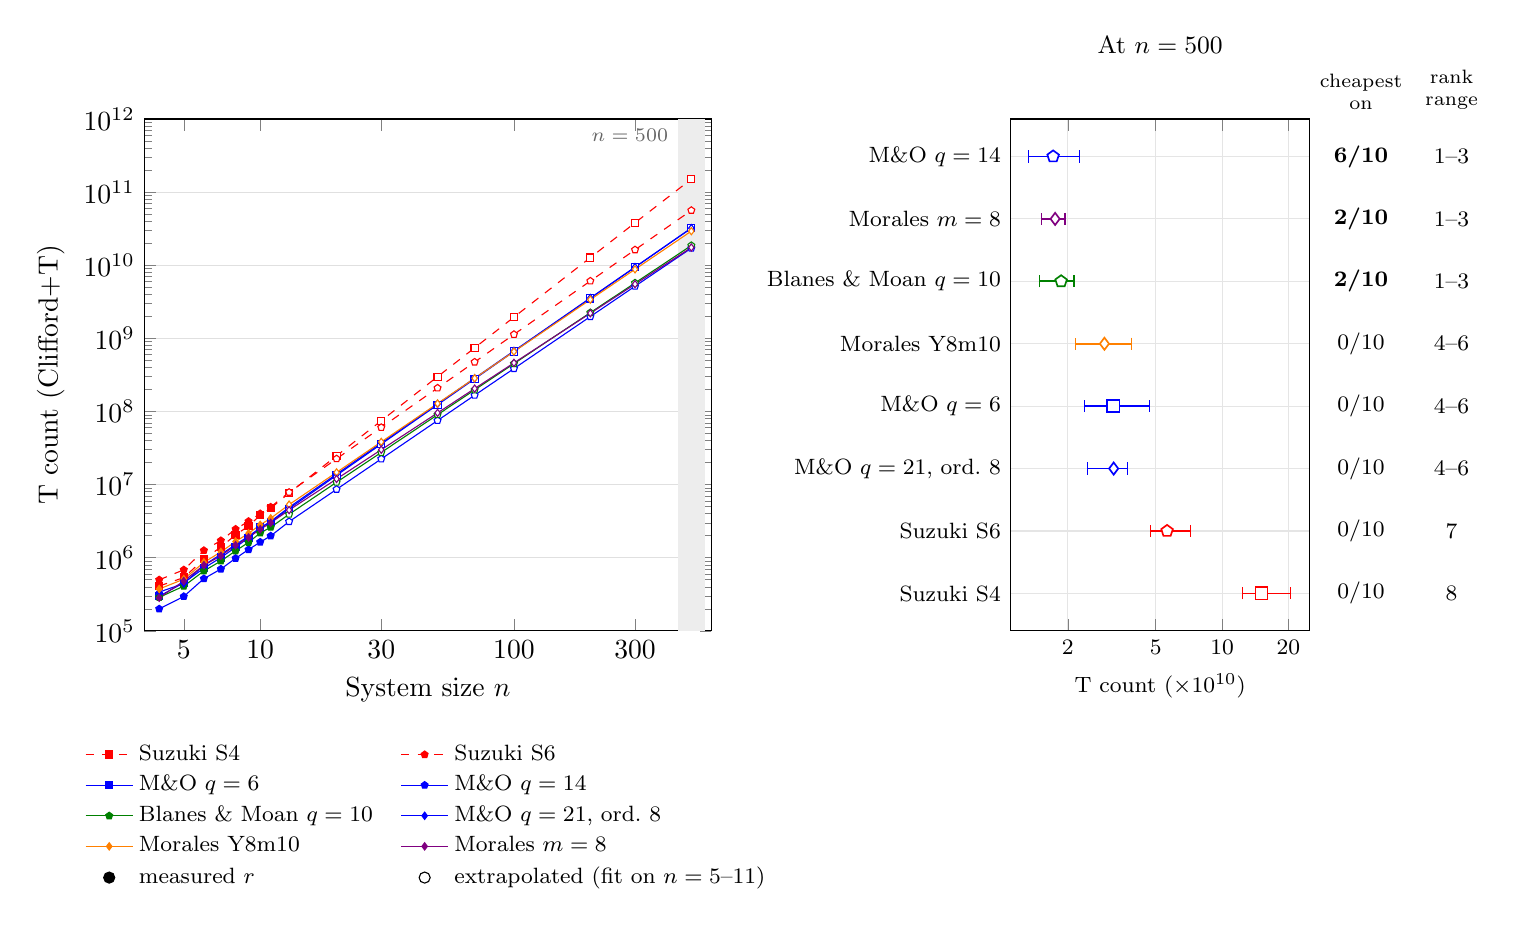
\begin{tikzpicture}
  \begin{loglogaxis}[
    name=main, scale only axis,
    width=7.2cm, height=6.5cm,
    xlabel={System size $n$},
    ylabel={T count (Clifford+T)},
    xtick={5,10,30,100,300}, xticklabels={5,10,30,100,300},
    xmin=3.5, xmax=600, ymin=100000, ymax=1e+12,
    ymajorgrids=true, grid style={black!12},
    legend style={at={(0.5,-0.2)}, anchor=north, draw=none, font=\footnotesize,
      legend columns=2, /tikz/every even column/.append style={column sep=8pt}},
    legend cell align=left,
  ]
    \fill[black!7] (axis cs:442.478,100000) rectangle (axis cs:565,1e+12);
    \node[anchor=north east, font=\scriptsize, black!60] at (axis cs:442.478,1e+12) {$n=500$};
    % suzuki4: measured n, mean over seeds, bars min..max over seeds
    \addplot[red, dashed, mark=square*, mark size=1.3pt, mark options={solid, fill=red}] coordinates {
      (4,410227)
      (5,535141)
      (6,956087)
      (7,1.39859e+06)
      (8,2.05215e+06)
      (9,2.71254e+06)
      (10,3.81418e+06)
      (11,4.74467e+06)
    };
    \addlegendentry{Suzuki S4}
    % suzuki4: extrapolated, per-seed fitted r, every step synthesised; mean over seeds, bars min..max
    \addplot[red, dashed, mark=square*, mark size=1.3pt, mark options={solid, fill=white}, mark indices={2,...,10}, forget plot] coordinates {
      (11,4.74467e+06)
      (13,7.66257e+06)
      (20,2.47721e+07)
      (30,7.47488e+07)
      (50,2.99557e+08)
      (70,7.41804e+08)
      (100,1.95329e+09)
      (200,1.27159e+10)
      (300,3.81078e+10)
      (500,1.5088e+11)
    };
    % suzuki6: measured n, mean over seeds, bars min..max over seeds
    \addplot[red, dashed, mark=pentagon*, mark size=1.3pt, mark options={solid, fill=red}] coordinates {
      (4,498655)
      (5,683636)
      (6,1.25709e+06)
      (7,1.71681e+06)
      (8,2.46342e+06)
      (9,3.14791e+06)
      (10,4.01292e+06)
      (11,4.938e+06)
    };
    \addlegendentry{Suzuki S6}
    % suzuki6: extrapolated, per-seed fitted r, every step synthesised; mean over seeds, bars min..max
    \addplot[red, dashed, mark=pentagon*, mark size=1.3pt, mark options={solid, fill=white}, mark indices={2,...,10}, forget plot] coordinates {
      (11,4.938e+06)
      (13,7.85273e+06)
      (20,2.25571e+07)
      (30,6.05362e+07)
      (50,2.09429e+08)
      (70,4.74592e+08)
      (100,1.13273e+09)
      (200,6.08751e+09)
      (300,1.62764e+10)
      (500,5.631e+10)
    };
    % mo-q6: measured n, mean over seeds, bars min..max over seeds
    \addplot[blue, solid, mark=square*, mark size=1.3pt, mark options={solid, fill=blue}] coordinates {
      (4,298204)
      (5,454337)
      (6,719342)
      (7,1.00507e+06)
      (8,1.38971e+06)
      (9,1.87541e+06)
      (10,2.57989e+06)
      (11,3.07213e+06)
    };
    \addlegendentry{M\&O $q=6$}
    % mo-q6: extrapolated, per-seed fitted r, every step synthesised; mean over seeds, bars min..max
    \addplot[blue, solid, mark=square*, mark size=1.3pt, mark options={solid, fill=white}, mark indices={2,...,10}, forget plot] coordinates {
      (11,3.07213e+06)
      (13,4.68293e+06)
      (20,1.33975e+07)
      (30,3.58209e+07)
      (50,1.23593e+08)
      (70,2.79089e+08)
      (100,6.61509e+08)
      (200,3.52821e+09)
      (300,9.37974e+09)
      (500,3.21589e+10)
    };
    % mo-q14: measured n, mean over seeds, bars min..max over seeds
    \addplot[blue, solid, mark=pentagon*, mark size=1.3pt, mark options={solid, fill=blue}] coordinates {
      (4,199644)
      (5,295456)
      (6,517803)
      (7,700110)
      (8,982626)
      (9,1.29212e+06)
      (10,1.63772e+06)
      (11,1.98699e+06)
    };
    \addlegendentry{M\&O $q=14$}
    % mo-q14: extrapolated, per-seed fitted r, every step synthesised; mean over seeds, bars min..max
    \addplot[blue, solid, mark=pentagon*, mark size=1.3pt, mark options={solid, fill=white}, mark indices={2,...,10}, forget plot] coordinates {
      (11,1.98699e+06)
      (13,3.11874e+06)
      (20,8.61978e+06)
      (30,2.2459e+07)
      (50,7.52655e+07)
      (70,1.66795e+08)
      (100,3.86553e+08)
      (200,1.98691e+09)
      (300,5.16555e+09)
      (500,1.71426e+10)
    };
    % bm-q10: measured n, mean over seeds, bars min..max over seeds
    \addplot[green!50!black, solid, mark=pentagon*, mark size=1.3pt, mark options={solid, fill=green!50!black}] coordinates {
      (4,287233)
      (5,408923)
      (6,658784)
      (7,901238)
      (8,1.23945e+06)
      (9,1.62436e+06)
      (10,2.1788e+06)
      (11,2.60871e+06)
    };
    \addlegendentry{Blanes \& Moan $q=10$}
    % bm-q10: extrapolated, per-seed fitted r, every step synthesised; mean over seeds, bars min..max
    \addplot[green!50!black, solid, mark=pentagon*, mark size=1.3pt, mark options={solid, fill=white}, mark indices={2,...,10}, forget plot] coordinates {
      (11,2.60871e+06)
      (13,3.9301e+06)
      (20,1.0774e+07)
      (30,2.7548e+07)
      (50,9.03062e+07)
      (70,1.9751e+08)
      (100,4.51462e+08)
      (200,2.24975e+09)
      (300,5.73099e+09)
      (500,1.86331e+10)
    };
    % mo-o8-q21: measured n, mean over seeds, bars min..max over seeds
    \addplot[blue, solid, mark=diamond*, mark size=1.3pt, mark options={solid, fill=blue}] coordinates {
      (4,338991)
      (5,443831)
      (6,791120)
      (7,1.1119e+06)
      (8,1.50621e+06)
      (9,1.97285e+06)
      (10,2.54893e+06)
      (11,3.13956e+06)
    };
    \addlegendentry{M\&O $q=21$, ord.~8}
    % mo-o8-q21: extrapolated, per-seed fitted r, every step synthesised; mean over seeds, bars min..max
    \addplot[blue, solid, mark=diamond*, mark size=1.3pt, mark options={solid, fill=white}, mark indices={2,...,10}, forget plot] coordinates {
      (11,3.13956e+06)
      (13,4.88976e+06)
      (20,1.39079e+07)
      (30,3.70353e+07)
      (50,1.2702e+08)
      (70,2.85327e+08)
      (100,6.73578e+08)
      (200,3.56917e+09)
      (300,9.45042e+09)
      (500,3.22461e+10)
    };
    % morales-y8m10: measured n, mean over seeds, bars min..max over seeds
    \addplot[orange, solid, mark=diamond*, mark size=1.3pt, mark options={solid, fill=orange}] coordinates {
      (4,373838)
      (5,509327)
      (6,864458)
      (7,1.19952e+06)
      (8,1.66587e+06)
      (9,2.15577e+06)
      (10,2.81799e+06)
      (11,3.46189e+06)
    };
    \addlegendentry{Morales Y8m10}
    % morales-y8m10: extrapolated, per-seed fitted r, every step synthesised; mean over seeds, bars min..max
    \addplot[orange, solid, mark=diamond*, mark size=1.3pt, mark options={solid, fill=white}, mark indices={2,...,10}, forget plot] coordinates {
      (11,3.46189e+06)
      (13,5.32463e+06)
      (20,1.47085e+07)
      (30,3.84186e+07)
      (50,1.28596e+08)
      (70,2.84865e+08)
      (100,6.59306e+08)
      (200,3.39046e+09)
      (300,8.80299e+09)
      (500,2.92891e+10)
    };
    % morales-m8: measured n, mean over seeds, bars min..max over seeds
    \addplot[violet, solid, mark=diamond*, mark size=1.3pt, mark options={solid, fill=violet}] coordinates {
      (4,283483)
      (5,480273)
      (6,790926)
      (7,1.06227e+06)
      (8,1.48074e+06)
      (9,1.89288e+06)
      (10,2.4461e+06)
      (11,3.00394e+06)
    };
    \addlegendentry{Morales $m=8$}
    % morales-m8: extrapolated, per-seed fitted r, every step synthesised; mean over seeds, bars min..max
    \addplot[violet, solid, mark=diamond*, mark size=1.3pt, mark options={solid, fill=white}, mark indices={2,...,10}, forget plot] coordinates {
      (11,3.00394e+06)
      (13,4.48114e+06)
      (20,1.19454e+07)
      (30,3.00095e+07)
      (50,9.5688e+07)
      (70,2.05711e+08)
      (100,4.61972e+08)
      (200,2.2065e+09)
      (300,5.51227e+09)
      (500,1.75035e+10)
    };
    \addlegendimage{only marks, black, mark=*, mark options={solid, fill=black}}
    \addlegendentry{measured $r$}
    \addlegendimage{only marks, black, mark=*, mark options={solid, fill=white}}
    \addlegendentry{extrapolated (fit on $n = 5$--$11$)}
  \end{loglogaxis}
  \begin{semilogxaxis}[
    scale only axis, clip=false,
    at={(11.0cm,0cm)}, anchor=south west,
    width=3.8cm, height=6.5cm,
    title={At $n = 500$}, title style={font=\small, yshift=14pt},
    xlabel={T count ($\times 10^{10}$)}, xlabel style={font=\footnotesize},
    xmin=1.1e+10, xmax=2.5e+11, xtick={2e+10,5e+10,1e+11,2e+11}, xticklabels={2,5,10,20},
    xminorticks=false,
    y dir=reverse, ymin=0.4, ymax=8.6, ytick={1,2,3,4,5,6,7,8},
    yticklabels={{M\&O $q=14$},{Morales $m=8$},{Blanes \& Moan $q=10$},{Morales Y8m10},{M\&O $q=6$},{M\&O $q=21$, ord.~8},{Suzuki S6},{Suzuki S4}},
    tick label style={font=\footnotesize}, ytick style={draw=none},
    xmajorgrids=true, ymajorgrids=true, grid style={black!10},
  ]
    % mo-q14: plotted 1.71426e+10, seeds 1.33055e+10..2.2523e+10, cheapest on 6/10, rank 1..3
    \addplot[blue, only marks, mark=pentagon*, mark size=2.2pt, mark options={solid, fill=white, line width=0.6pt}, error bars/.cd, x dir=both, x explicit, error bar style={solid, line width=0.6pt}] coordinates {
      (1.71426e+10,1) += (5.38038e+09,0) -= (3.83706e+09,0)
    };
    % morales-m8: plotted 1.75035e+10, seeds 1.51658e+10..1.94095e+10, cheapest on 2/10, rank 1..3
    \addplot[violet, only marks, mark=diamond*, mark size=2.2pt, mark options={solid, fill=white, line width=0.6pt}, error bars/.cd, x dir=both, x explicit, error bar style={solid, line width=0.6pt}] coordinates {
      (1.75035e+10,2) += (1.90596e+09,0) -= (2.33772e+09,0)
    };
    % bm-q10: plotted 1.86331e+10, seeds 1.48173e+10..2.13136e+10, cheapest on 2/10, rank 1..3
    \addplot[green!50!black, only marks, mark=pentagon*, mark size=2.2pt, mark options={solid, fill=white, line width=0.6pt}, error bars/.cd, x dir=both, x explicit, error bar style={solid, line width=0.6pt}] coordinates {
      (1.86331e+10,3) += (2.68049e+09,0) -= (3.81581e+09,0)
    };
    % morales-y8m10: plotted 2.92891e+10, seeds 2.17099e+10..3.88229e+10, cheapest on 0/10, rank 4..6
    \addplot[orange, only marks, mark=diamond*, mark size=2.2pt, mark options={solid, fill=white, line width=0.6pt}, error bars/.cd, x dir=both, x explicit, error bar style={solid, line width=0.6pt}] coordinates {
      (2.92891e+10,4) += (9.53382e+09,0) -= (7.5792e+09,0)
    };
    % mo-q6: plotted 3.21589e+10, seeds 2.37233e+10..4.7055e+10, cheapest on 0/10, rank 4..6
    \addplot[blue, only marks, mark=square*, mark size=2.2pt, mark options={solid, fill=white, line width=0.6pt}, error bars/.cd, x dir=both, x explicit, error bar style={solid, line width=0.6pt}] coordinates {
      (3.21589e+10,5) += (1.48961e+10,0) -= (8.4356e+09,0)
    };
    % mo-o8-q21: plotted 3.22461e+10, seeds 2.46524e+10..3.74206e+10, cheapest on 0/10, rank 4..6
    \addplot[blue, only marks, mark=diamond*, mark size=2.2pt, mark options={solid, fill=white, line width=0.6pt}, error bars/.cd, x dir=both, x explicit, error bar style={solid, line width=0.6pt}] coordinates {
      (3.22461e+10,6) += (5.17455e+09,0) -= (7.59363e+09,0)
    };
    % suzuki6: plotted 5.631e+10, seeds 4.74716e+10..7.17507e+10, cheapest on 0/10, rank 7..7
    \addplot[red, only marks, mark=pentagon*, mark size=2.2pt, mark options={solid, fill=white, line width=0.6pt}, error bars/.cd, x dir=both, x explicit, error bar style={solid, line width=0.6pt}] coordinates {
      (5.631e+10,7) += (1.54407e+10,0) -= (8.83844e+09,0)
    };
    % suzuki4: plotted 1.5088e+11, seeds 1.23785e+11..2.03957e+11, cheapest on 0/10, rank 8..8
    \addplot[red, only marks, mark=square*, mark size=2.2pt, mark options={solid, fill=white, line width=0.6pt}, error bars/.cd, x dir=both, x explicit, error bar style={solid, line width=0.6pt}] coordinates {
      (1.5088e+11,8) += (5.3077e+10,0) -= (2.70956e+10,0)
    };
    \node[anchor=south, font=\scriptsize, align=center] at ([xshift=0.65cm]axis cs:2.5e+11,0.4) {cheapest\\on};
    \node[anchor=south, font=\scriptsize, align=center] at ([xshift=1.8cm]axis cs:2.5e+11,0.4) {rank\\range};
    \node[font=\footnotesize\bfseries] at ([xshift=0.65cm]axis cs:2.5e+11,1) {6/10};
    \node[font=\footnotesize] at ([xshift=1.8cm]axis cs:2.5e+11,1) {1--3};
    \node[font=\footnotesize\bfseries] at ([xshift=0.65cm]axis cs:2.5e+11,2) {2/10};
    \node[font=\footnotesize] at ([xshift=1.8cm]axis cs:2.5e+11,2) {1--3};
    \node[font=\footnotesize\bfseries] at ([xshift=0.65cm]axis cs:2.5e+11,3) {2/10};
    \node[font=\footnotesize] at ([xshift=1.8cm]axis cs:2.5e+11,3) {1--3};
    \node[font=\footnotesize] at ([xshift=0.65cm]axis cs:2.5e+11,4) {0/10};
    \node[font=\footnotesize] at ([xshift=1.8cm]axis cs:2.5e+11,4) {4--6};
    \node[font=\footnotesize] at ([xshift=0.65cm]axis cs:2.5e+11,5) {0/10};
    \node[font=\footnotesize] at ([xshift=1.8cm]axis cs:2.5e+11,5) {4--6};
    \node[font=\footnotesize] at ([xshift=0.65cm]axis cs:2.5e+11,6) {0/10};
    \node[font=\footnotesize] at ([xshift=1.8cm]axis cs:2.5e+11,6) {4--6};
    \node[font=\footnotesize] at ([xshift=0.65cm]axis cs:2.5e+11,7) {0/10};
    \node[font=\footnotesize] at ([xshift=1.8cm]axis cs:2.5e+11,7) {7};
    \node[font=\footnotesize] at ([xshift=0.65cm]axis cs:2.5e+11,8) {0/10};
    \node[font=\footnotesize] at ([xshift=1.8cm]axis cs:2.5e+11,8) {8};
  \end{semilogxaxis}
\end{tikzpicture}
